\chapter{Technical Details}

\section{Methodology}

\subsection{Dataset}
\integrity{JL}{QH} Based on our literature review in \autoref{sec:existing_works}, we identified weather, traffic events, and traffic speed as key factors for predicting traffic flow. Thus, we are collecting datasets from the following sources:
\begin{itemize}
    \item Traffic events: 511.org
    \item Weather: OpenWeather
    \item Traffic speed: Caltrans Performance Measurement System (PeMS)
\end{itemize}

For weather and traffic event data, it is easier for us to get data because they provide API to call directly. Therefore, we can get data at the frequency we want, which is every 5 minutes. However, PeMS does not allow users to crawl their data frequently without their permission. Therefore, we choose to download PeMS daily data every day instead of every 5 minutes.

\subsection{Traffic Modeling}
\integrity{NK}{QH}
At the start of the project, we gathered data from various sources, merged it, and assigned a section ID to each segment of I-880 for which predictions were to be made. This consolidated dataset was then subjected to exploratory data analysis (EDA) to assess its structure, identify missing values, and detect outliers. We performed data cleaning by eliminating irrelevant columns and data points through this process. The analysis used data on current traffic speeds, weather conditions, incidents, calendar dates, and times. We applied one-hot encoding to the categorical variables, such as weather conditions, traffic incidents, calendar dates, and times, and standardized the numerical data, such as current traffic speeds.
In our feature engineering phase, we identified the most critical severity for events that occurred within a 60-minute window before the forecast time and within a 10-mile radius of the midpoint of the predicted section. We then introduced a new feature called the event severity score, which was calculated using the following formula:

\begin{equation}
    \text{Severity Score} = \text{severity} \times \left( e^{-\text{time}} + e^{-\text{distance}} \right)
\end{equation}

For weather and traffic event data, where there were many types, and the individual impact was unclear, related categories were consolidated. Additionally, Principal Component Analysis (PCA) was applied to the entire dataset to reduce the dimensionality of the features. These preprocessing techniques aimed to enhance the efficiency of model training and the accuracy of forecasts.
In constructing the traffic flow forecasting model, linear regression, random forest, LightGBM, and a neural network MLP (Multilayer Perceptron) were compared. The model with the lowest MSE was chosen as the final model.

\subsection{Cloud Computing}
\integrity{QH}{JL} Our pipeline will utilize the Google Cloud Platforms. We aim to 
\begin{enumerate}
    \item Establish a production-grade data pipeline, incorporating data collection, processing, inference, and visualization.
    \item Introduce data replay capabilities for a faster review of historical changes.
    \item Support streaming data to observe real-time changes.
\end{enumerate}

Our focus lies on utilizing FaaS (Function as a Service) for project implementation and deployment to scale down running and maintenance costs. We exchange real-time data via Pub/Sub, a publisher-subscriber system, while data storage is handled by BigQuery, a data warehouse. Our implementation consists of the following components:

\begin{enumerate}
    \item Data Ingestors/Replayer: We will employ Cloud Function to ingest data from the datasets or to replay data from BigQuery. These processes are triggered using Cloud Scheduler based on specified inputs.
    \item Preprocessor: We will preprocess the data using the feature engineering techniques detailed in the previous section, facilitated by Dataflow.
    \item Inference: Depending on the scale of our model, the inference will run on either Dataflow or Cloud Function.
    \item Dashboard: Dashboards will be deployed via Cloud Run which we will discuss in a subsequent section.
\end{enumerate}

\subsection{Dashboard}
\integrity{JL}{QH} To enhance the visualization of predictive traffic flow and streamline development efforts, we have chosen Grafana, a robust visualization tool, to present our model predictions. Grafana offers a wide range of plot types, including time series, bar charts, heatmaps, and geomaps, making it a versatile choice. Additionally, its support for various plugins allows seamless integration with different databases. In our implementation, we incorporated the BigQuery plugin to facilitate connection with our dataset, empowering Grafana to generate insightful visualizations.

The first section of our dashboard focuses on time series data for individual segments. This includes the actual observed speeds sourced from PeMS data alongside our predictive values. To enrich the analysis, we've integrated event scores onto these graphs. These visualizations enable us not only to compare predicted and actual speeds but also to examine any correlation between event scores and actual speed fluctuations.

The second segment of the dashboard is dedicated to showcasing traffic congestion levels on a geographical map. This provides users with a comprehensive view of congestion across different segments at specific timestamps. Each segment is represented by an arrow on the map, with colors indicating the severity of congestion. As congestion escalates, the color of the arrow transitions from green to orange, red, and eventually purple, providing a clear indication of worsening traffic conditions.
 

\subsection{Low-code approach}
\integrity{JL}{QH} In order to illustrate the concept of our low-code framework, we plan to reverse engineer our implementation. This will transform our product into a reference architecture and a domain-specific language (DSL). Our low-code framework design is supported by the reference architecture, which functions as the fundamental backbone. In this proposed design, the low-code framework will be responsible for generating the application code using our reference architecture. 

Our DSL has been formulated to combat the issues associated with traditional approaches such as SQL, which grapple with stateful transformations, late or out-of-order data, and trade-offs between cost, correctness, and latency. The DSL will be specified in pseudocode, using Python as the designated language. 

Our core objectives in this methodology are to incorporate the separation of the data model and control flow, ensure the proficient use of decorators, and define stateful and stateless transformations in a more straightforward and efficient manner.

\section{Results}
\subsection{Traffic Modeling: Accuracy}
\integrity{NK}{QH} Initially, as a baseline, the Mean Squared Error (MSE) was computed using the current speed as the forecasted speed for 10 minutes later, without any modifications. Subsequently, the results of the comparative analysis using linear regression, random forest, LightGBM, and MLP neural networks, which are utilized in other studies mentioned in the literature review, revealed that the MLP model exhibited superior performance, as indicated in the table ~\ref{table:mse_comparison_transposed}. Model training and accuracy evaluation were conducted using five-fold cross-validation and MSE, and hyperparameter optimization was carried out using random search. The MLP model achieved an 11.8\% reduction in MSE compared to the baseline. Furthermore, the MLP model reduced the MSE by 7.8 \% compared to a fundamental linear regression benchmark, offering more realistic forecasts than the other evaluated models.

\begin{table}[ht]
\centering
\begin{tabular}{c|c|c|c|c|c}
 &Base Line & Linear Regression & Random Forest & LightGBM & MLP \\ \hline
MSE & 2.80 &2.68 & 2.62 & 2.51 & 2.47
\end{tabular}
\caption{Comparison of MSE with 5-Fold Across Various Models}
\label{table:mse_comparison_transposed}
\end{table}

\subsection{Cloud Computing}
\integrity{QH}{JL} Through the use of serverless compute technologies, our implementation on the Google Cloud Platform supports streaming data processing, facilitated by the use of PubSub and Dataflow. This functionality means that our pipeline can be evaluated against real-time data, enabling users to conduct analyses based on real-time inputs rather than relying solely on downloaded data. Specifically, our pipeline can generate real-time predictions of traffic speeds for the next 10 minutes based on current data.

Additionally, due to the adoption of FaaS, our implementation requires minimal maintenance once deployed and hence, incurs minimal costs. As Google manages the fundamental environment for our implementation, we eliminate the need to handle the complex setup of operating systems and environment. Furthermore, Google will only bill us for the time resources are in use, thereby reducing wastage of funds on idle resources. On average, our implementation incurs approximately \$0.50 in costs per day.

\subsection{Dashboard}
\integrity{JL}{QH} Our dashboard is shown below in  \autoref{fig:dashboard}, which provides a time-series view on specific data for each segment, and a map-view on overall congestion level for all segments given a specific time.

In examining the time series panel, two noteworthy observations emerge. Firstly, our predictions consistently lag behind the actual speed. This discrepancy arises because our model forecasts the speed 10 minutes ahead based mostly on the current speed, essentially employing a baseline approach. This allows us to assess the accuracy of our model in comparison to this baseline. Secondly, the event score appears disconnected from instances of speed drops. Potential explanations for this misalignment include inaccuracies in the formula used to calculate the event score or discrepancies in the event data itself. Upon investigation, we discovered instances where event data from 511.org may be sourced from alternative channels, resulting in multiple events sharing identical creation times. This suggests a potential need for refining the event data collection process to ensure accuracy. Moreover, even when creation times are intended to be accurate, delays between the occurrence of an event and its reporting may still impact the data reliability.

Turning to the map panel, a notable disparity in congestion levels between peak traffic hours and midnight is evident. Users have the flexibility to adjust the time settings to observe distinct patterns. 

\begin{figure}
    \centering
    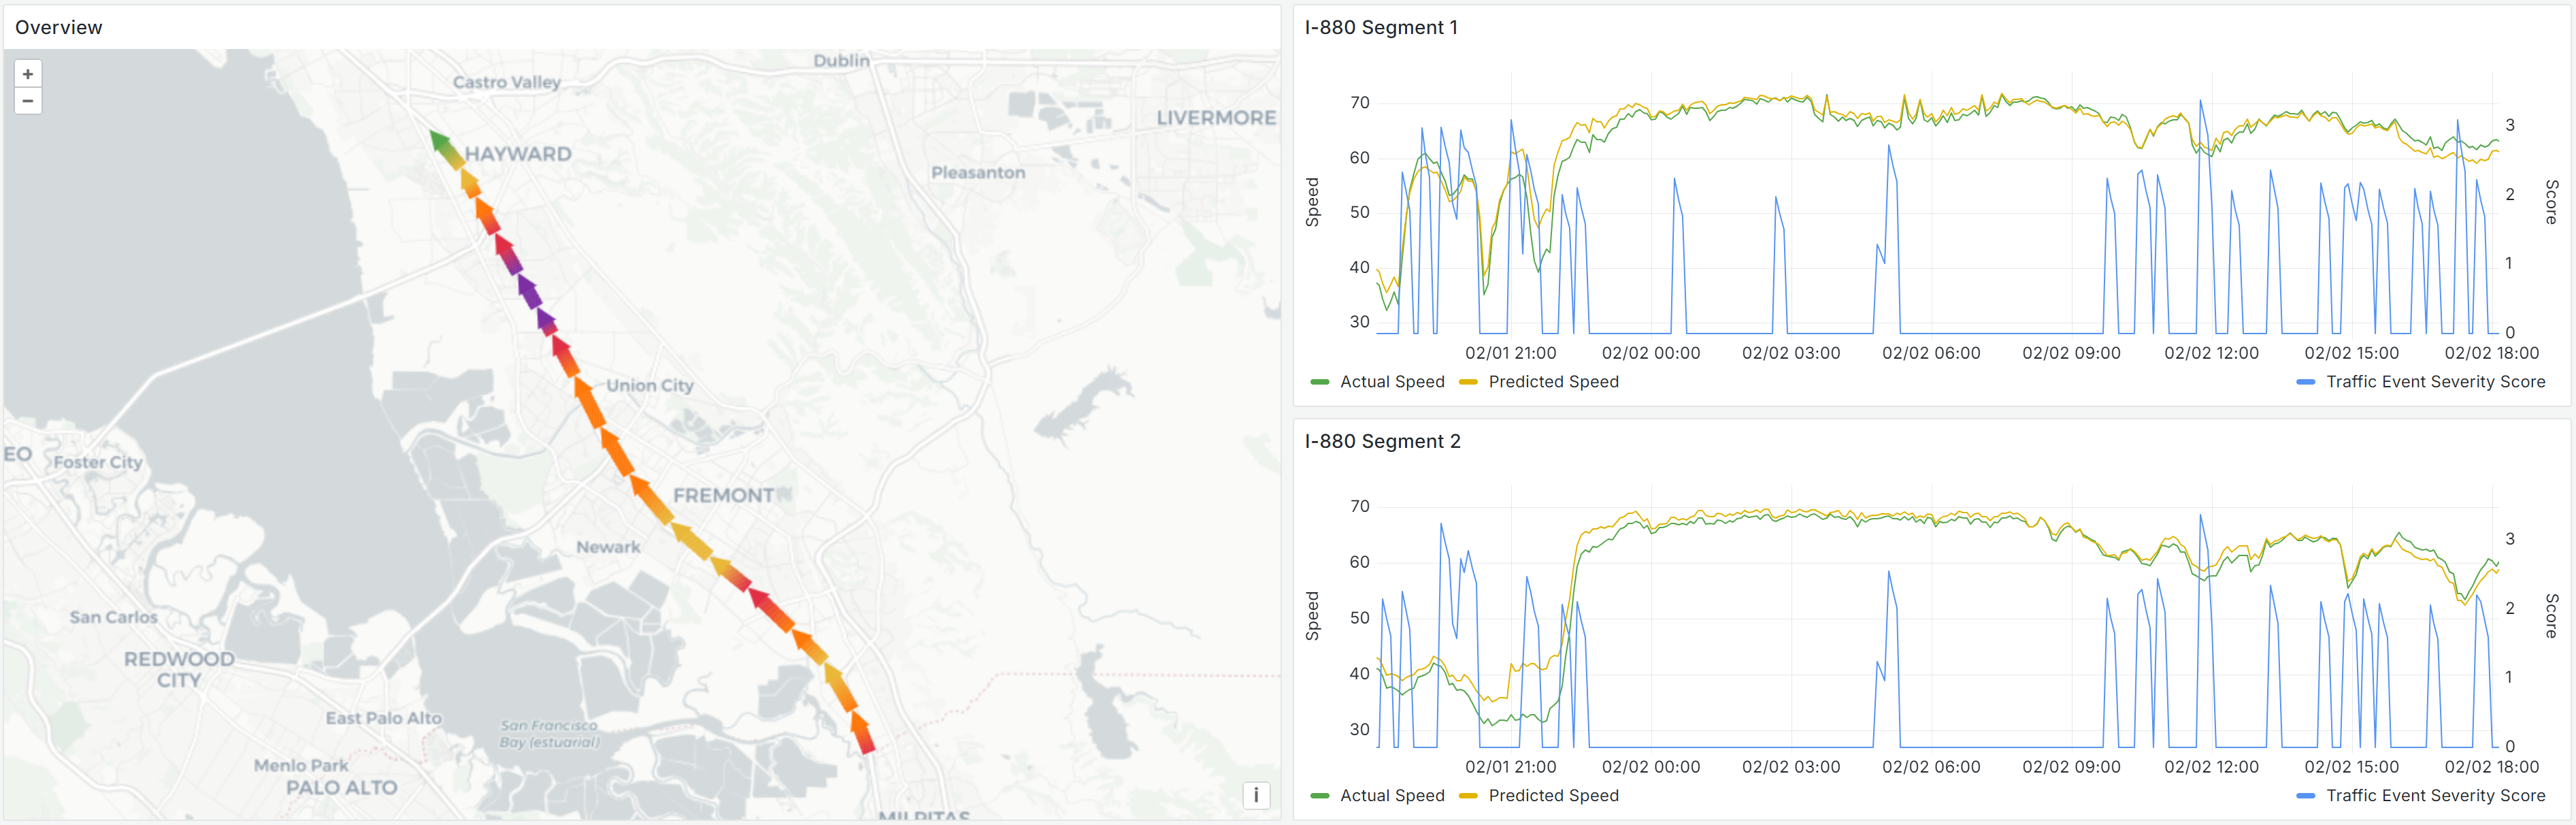
\includegraphics[width=\textwidth]{img/dashboard.png}
    \caption{Dashboards for I-880}
    \label{fig:dashboard}
\end{figure}

\subsection{Reference Architecture} 
\integrity{QH}{JL} By reverse-engineering our implementation, we have created a reference architecture, as shown below, for general-purpose digital-twin applications. Based on our business analysis, our reference architecture reflects our implementation by dividing the product into several components: data ingestors, data replayers, feature pipeline, training pipeline, inference pipeline, and business insights. We distinguished between functionality and technology by representing the required technology within the boxes. Our low-code framework will mirror this design when generating the application code.

\begin{figure}
    \centering
    \includesvg[width=\textwidth]{img/ref_arch.svg}
    \caption{Reference Architecture}
    \label{fig:ref_arch}
\end{figure}
\subsection{Domain Specific Languages}

\integrity{JL}{QH} The DSL design comprises two main components. Firstly, we conceptualize data as assets organized into typed streams, allowing for easier transformation through framework built-in functions. Secondly, our DSL incorporates default stream operations to enhance operational efficiency.

For typed streams, we define sample, event, session, transition, and journal. These typed data models' features and descriptions are detailed in \autoref{table:data-model}.

\begin{table}[ht]
\centering
\begin{tabular}{c|c|c}
    Model Type & Features & Example \\ \hline 
    Sample & Near-periodic Timestamps & Teamperature Measurements \\
    Event & Non-periodic Timestamps, Typed or untyped events & Alerts from monitoring systems \\
    Session & Start \& end times, Non-overlapping intervals & Machine production runs \\
    Transition & Time-partitioning & Parking space availability \\
    Journal & Strictly periodic timestamps, Sliding or tumbling window & Daily sales reports
\end{tabular}
\caption{Comparison of MSE with 5-Fold Across Various Models}
\label{table:data-model}
\end{table}

Regarding stream operations, we define multiple types, including operations within a stream and among multiple streams. Our design assumes that all data types can be accommodated within typed streams, and data transformation and feature pipeline operations can be executed seamlessly using our operation design. For operations within a stream, we specify 
\begin{itemize}
    \item {\tt map}: 1-1 record transformation
    \item {\tt filter}: record filtering
    \item {\tt splitter}: record splitting
    \item {\tt window}: time window-based record selection
    \item {\tt groupby}: grouping records by key with aggregate functions
\end{itemize}
Operations among multiple streams include 
\begin{itemize}
    \item {\tt union}: combining streams without joining
    \item {\tt dispatch}: one-to-many stream splitting
    \item {\tt join}: merging streams based on key and/or timestamp
\end{itemize}


Although the example of DSL implementation is ongoing and will be added later, our initial implementation utilizes DSL for feature pipeline and inference, notably Dataflow. Hence, we plan to compare our DSL with Dataflow to evaluate its usability and practicality. An example of the comparison is shown in \autoref{fig:comparison}.

Overall, our implementation serves as evidence of the practicality of a low-code framework. If users can easily write code of this nature, the framework could seamlessly translate it into a reference architecture and generate corresponding components within a cloud environment. We envision this level of abstraction as accessible for individuals with a basic coding proficiency but lacking extensive software and data engineering backgrounds, enabling them to develop data-intensive applications.

Further refinement and expansion of our project's technical aspects are slated for future implementation.

\begin{landscape}
\begin{figure}
    \centering
  \begin{minipage}[t]{.45\linewidth}
\begin{minted}[linenos]{python}
for segment in get_metadata()['segments']:
    # fetch weather data for each of the segment
    lat = segment["representative_point"][0]
    lon = segment["representative_point"][1]

    response = requests.get(API_ENDPOINT, params={
        "lon": lon,
        "lat": lat,
        "appid": os.environ['API_KEY'],
        "units": "metric",
    })
    response.raise_for_status()
    proto = ParseDict(response.json(), Weather())

    publisher_client = pubsub.PublisherClient()
    topic_path = publisher_client.topic_path(
        os.environ['PROJECT_ID'], os.environ['TOPIC_ID'])
    publisher_client.publish(
        topic_path, proto.SerializeToString())
\end{minted}
\end{minipage}
\begin{minipage}[t]{.45\linewidth}
\begin{minted}[linenos]{python}
city = City(name="Berkeley", lat=20.0, lon=25.0)
weather = Weather.from_source(city)
speed = SpeedSample.from_source([
    PeMSStation(id=50000), PeMSStation(id=50001)])
events = EventSample.from_source()

sessionizer = Sessionizer(EventSample, EventSession, feature="event_id")

events.data[['Severity']] # pandas
\end{minted}
\end{minipage}  
    \caption{Comparison between DSL and Dataflow Implementation}
    \label{fig:comparison}
\end{figure}
\end{landscape}

\section{Future Work}
\subsection{Low-code Framework}

\integrity{QH}{JL} While our project has proposed a viable method for implementing a low-code framework through our Domain-Specific Language (DSL) and reference architecture, the actual development within Anaximander--the low-code framework we are developing--remains a work in progress. To fully realize the potential of our work for Anaximander, we will need to establish a transformation process from our DSL to executable code. Additionally, it will be necessary to interconnect different components using code, and develop tools that enable users to easily manage them, to ensure compatibility with our reference architecture and fulfill our project's objectives.

\subsection{Model Improvements and Data Correctness}
\integrity{NK}{OH} The accuracy is crucial to the usefulness of this application. In order to improve the accuracy, future efforts will focus on getting more high-quality data or enhancing the model. On the other hand, model enhancements will require a more detailed redefinition of event severity, improved feature engineering and selection, and the exploration of deep learning architectures designed explicitly for time-series forecasting. The most significant events are identified within a 60-minute window preceding the forecast time and within a 10-mile radius of the forecast interval's midpoint. However, a finer temporal and spatial refinement of the event severity definition could provide a more nuanced understanding of the relationship between events and velocity.
Furthermore, the accuracy can be improved by adding and examining the correlation between different speeds (fast, medium, and slow) and forecasts. Moreover, the model can reduce complexity and prevent overfitting by eliminating less relevant ones. Additionally, it will investigate deep learning architectures and techniques, including RNNs suitable for time-series analysis, enhanced versions like LSTM and GRU, and the statistical time series model SARIMA. These improvements will be implemented incrementally in stages to enhance the accuracy and reliability of our forecasting models.

\subsection{Continuous Training Using Streaming Data}

\integrity{QH}{JL} Continuous improvement of models is another crucial aspect to consider for many business purposes, due to the constantly changing trends in users' behaviors and needs. To incorporate this concept, our reference architecture will need updates to include components that allow for such continuous improvements, whether locally or in the cloud. This could involve, for example, the addition of a model evaluation component and a model store. Additional logic may also be required, such as the continuous evaluation of model performance, complemented by dashboards that visualize relevant error metrics. Moreover, our Domain-Specific Language (DSL) would need updates to simplify processes for users. For instance, within our DSL, users could specify the frequency and dataset size necessary for model training, eliminating the need for writing complex scheduler logics.

\section{Conclusion}

\integrity{QH}{JL} Our project has comprehensively explored the challenge of digital-twin development involving IoT devices, specifically predicting traffic flow. We have gathered, analyzed, and modeled data from diverse sources, applying state-of-the-art machine learning techniques and leveraging cloud computing technologies to achieve our objectives. Through our efforts, we have not only developed a robust model for traffic flow prediction but also created a scalable, cost-effective infrastructure on the Google Cloud Platform, which stands as a reference implementation to the potential of low-code frameworks in handling big data and real-time analytics.

Our innovative approach in integrating a low-code framework and a Domain-Specific Language (DSL) creates an innovative strategy to democratize technology, making it accessible to people without software engineering expertise, such as domain experts and data scientists. Our project aligns with our vision to allow users to perform advanced analytics and machine learning without the need for deep technical knowledge.

\wordcount{report_section2}